\scanpage{95}
\mspage{15}
\deleted{more} simple, \unsure{which|that} for $I'=p^{-1}(I)$ does not depend on the choice of $I'$ i.e. of $I$. If one wants the lifted action $\Theta'$ to be the identity on $I'$, one has uniqueness, and the additional condition that $\widetilde{\Theta}$ must indeed act \uline{trivially} on $I'$.

Let us return: the action of $\Gamma$ \inserted{$=\operatorname{Gal}\overline{K}/K$} on a $\mathcal{C}=\deleted{\unsure{\Pi_1}}\widehat{\Pi}_1(X,I)$ with $I\subset X_K$, we therefore find a necessary condition for an automorphism $\Theta$ of $\mathcal{C}$ \inserted{trivial on the objects} to come from a $u\in\Gamma$:

\margin{These two conditions in fact depend only on the action of \deleted{$\Theta$} $\Theta$ on the fundamental group at \uline{one} point $x_0\in I$}
a) For every finite \inserted{étale} covering $X'$ of $X$, \inserted{(defined over $K$)} \deleted{\unsure{it considers}} \deleted{\unsure{there is} the action of} \inserted{there is an action $\widetilde{\Theta}$ of} $\Theta$ on $\widehat{\Pi}_1(X',I')$, where $I'=X'|I$, which lifts $\Theta$, and which is the identity on $I'\cap X'_K$.

b) Moreover, for $\forall$ homomorphism (defined over $K$)
\[
X'\xrightarrow{f}Y,
\]
and every $x'\in I'\cap X'_K$, the kernel of
\[
(*)\qquad\widehat{\Pi}_1(X',x')\longrightarrow\widehat{\Pi}_1(\unsure{Y|X},f x')
\]
is stable under $\widetilde{\Theta}^{\unsure{\prime|*}}$ \inserted{(for suitable $\widetilde{\Theta}$!)} --- more generally, without assuming $x'\in X'_K$, but choosing $\nu\in\mathbb{N}^{+}$ such that $\Theta^\nu x'=x'$, it is necessary that \deleted{$\Theta$} the kernel of $(*)$ be stable under $\Theta^\nu$.

\margin{\uline{NB} These conditions \deleted{\unsure{of}} unformulable, so long as we \unsure{confined|confine} ourselves to the point of view of the \uline{outer} actions of $\Gamma$!}
\figure{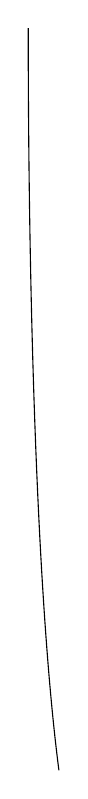
\begin{tikzpicture}[x=0.01cm,y=0.01cm]
\draw (0,0) .. controls (0,-320) and (10,-720) .. (39,-943);
\end{tikzpicture}}
These are draconian conditions. I \unsure{think|can} that I am not going too far,
\margin{94}
